% homework/hw05/hw05.tex
% Year 7 - Homework Packet 5: the whole of Unit 1, in one packet.
%
% Covers Science 1.1-1.4 (cells, animal cells, specialised cells, tissues and
% organs) and Mathematics 1.1-1.6 (integers, multiples and the LCM, factors and
% the HCF, tests for divisibility, squares, cubes and roots).
%
% Two things about this packet are deliberate and different from HW 1-4:
%
%   * SCIENCE COMES FIRST. Every other packet leads with maths. This one leads
%     with science because the science section is the shorter of the two and
%     the maths runs to five pages -- opening on the long one makes the packet
%     look unfinishable, and this is a review packet a student should want to
%     start.
%
%   * The maths is deliberately most of the packet, and most of the maths is
%     skills and word problems rather than new ideas. Unit 1 is finished; what
%     is left is fluency and, as always in this class, the English of the
%     question.
%
% Nothing is lifted from the workbook, and no question is a straight repeat of
% HW 1-4. Where a trap is reused it has new numbers and a new context: the
% "difference between -7 and 4" pair in B4 is HW 1's A4 trap with new numbers,
% and C2 is the LCM/HCF confusion that HW 2 and HW 3 could only test one at a
% time, now put side by side, which is where the class actually meets it.
%
% House style is shared: see homework/hw-style.tex. Method: the new-homework
% skill. Source is pure ASCII on purpose.
%
% Build:  pwsh .claude/skills/new-homework/scripts/build-hw.ps1 hw05

\documentclass[12pt,a4paper]{article}

% -- Answer key switch -------------------------------------------------------
\newif\ifkey
\ifdefined\TEACHER\keytrue\else
  \keyfalse        % \keyfalse = student copy   |   \keytrue = teacher copy
\fi

% -- House style -------------------------------------------------------------
% homework/hw-style.tex
% Shared house style for every Year 7 homework packet. \input this from the
% packet file, right after \documentclass and the answer-key switch.
%
% Do not fork this file per packet. If a packet needs a different look, the
% question is whether every packet should have it.
%
% The choices here are deliberate and were arrived at by printing and looking:
%   * No solid dark banners. Every header is a light tint with a coloured spine
%     on the left, so colour reads clearly without flooding a school printer.
%   * No marks and no mark totals. These are practice, not exam papers.
%   * Lato at 12pt with open leading, plus mathastext so inline maths is Lato
%     too. Without mathastext every "-6 + 4" is Computer Modern serif and the
%     sheet looks half-typeset.
%   * Writing lines are spaced for Year 7 handwriting, not adult margin notes.
%
% Provides: \wlines \blank \tickbox \sep \qmk-free marks (none) \hwsection
% \qhead \expr, the workspace box, and the remember / wordhelp / activity /
% yourturn coloured boxes. Palette matches the lesson decks exactly.

% -- Packages ----------------------------------------------------------------
\usepackage[T1]{fontenc}
\usepackage[utf8]{inputenc}
\usepackage[default]{lato}
\usepackage[a4paper,top=1.7cm,bottom=1.7cm,left=2.0cm,right=2.0cm,headheight=15pt]{geometry}
\usepackage{amsmath,amssymb}
\usepackage{xcolor}
\usepackage[most]{tcolorbox}
\usepackage{enumitem}
\usepackage{tikz}
\usetikzlibrary{arrows.meta}
\usepackage{array}
\usepackage{tabularx}
\usepackage{fancyhdr}
\usepackage{multicol}
\usepackage{needspace}
\usepackage{graphicx}

% Make maths use Lato too. Without this, every "-6 + 4" on the page is set in
% Computer Modern serif and the sheet looks half-typeset. Must come last.
\usepackage[italic]{mathastext}

\linespread{1.06}\selectfont

% -- The Learner's Book palette (same hex values as the lesson decks) ---------
\definecolor{cbteal}{HTML}{0087A8}
\definecolor{cbpurple}{HTML}{5C2483}
\definecolor{cborange}{HTML}{C25E12}
\definecolor{cbgreen}{HTML}{4A8B23}
\definecolor{cbred}{HTML}{C8102E}
\definecolor{cbblue}{HTML}{1A5FA8}
\definecolor{rulegray}{HTML}{9AA5AD}

% -- Answer lines and blanks -------------------------------------------------
% \wlines{n} draws n ruled writing lines, spaced wide enough for Year 7
% handwriting rather than for an adult with a fine pen.
\makeatletter
\newcommand{\wlines}[1]{%
  \par\vspace{0.75em}%
  \@tempcnta=0\relax
  \@whilenum\@tempcnta<#1\do{%
    \hbox to \linewidth{\color{rulegray}\leaders\hrule height 0.5pt\hfill}%
    \vspace{1.5em}%
    \advance\@tempcnta by 1\relax}%
  \par\vspace{-0.8em}%
}
\makeatother

% \blank[width] is an inline gap to write a short answer in.
\newcommand{\blank}[1][2.6cm]{\underline{\hspace{#1}}}

% A boxed space for showing working.
\newtcolorbox{workspace}[1][3.4cm]{%
  colback=white, colframe=rulegray, boxrule=0.5pt, arc=5pt,
  height=#1, left=6pt, right=6pt, top=4pt, bottom=4pt,
  before skip=9pt, after skip=11pt}

% An empty tick box.
\newcommand{\tickbox}{\fbox{\rule{0pt}{1.15em}\rule{1.15em}{0pt}}}

% A middot separator.
\newcommand{\sep}{\,\textperiodcentered\,}

% -- Section and question headings -------------------------------------------
% Light tint plus a fat coloured spine on the left. No solid dark banner: the
% colour reads clearly but barely costs the printer anything.
% needspace stops a heading stranding alone at the foot of a page. Kept modest:
% too large and it pushes headings over, leaving a worse hole than it prevents.
\newcommand{\hwsection}[2][cbteal]{%
  \needspace{8\baselineskip}%
  \par\vspace{13pt}%
  \noindent
  \begin{tcolorbox}[enhanced, nobeforeafter, width=\textwidth,
      colback=#1!7, colframe=#1!7, arc=5pt,
      borderline west={5pt}{0pt}{#1},
      left=14pt, right=10pt, top=7pt, bottom=7pt]
    {\large\bfseries\color{#1}#2}
  \end{tcolorbox}%
  \par\vspace{9pt}}

% \qhead[colour]{A2}{Moving along the line} -- a question heading.
\newcommand{\qhead}[3][cbteal]{%
  \needspace{6\baselineskip}%
  \par\vspace{11pt}%
  \noindent{\large\bfseries\color{#1}#2}\quad{\large\bfseries #3}\par\vspace{4pt}}

% -- Coloured boxes ----------------------------------------------------------
% Shared look: rounded, light fill, coloured rule, coloured title text on a
% pale title strip rather than a dark one.
\tcbset{hwbox/.style={
  enhanced, breakable, arc=6pt, boxrule=1pt,
  left=11pt, right=11pt, top=8pt, bottom=8pt,
  fonttitle=\bfseries, attach boxed title to top left={xshift=12pt, yshift=-8pt},
  boxed title style={arc=4pt, boxrule=1pt, left=7pt, right=7pt, top=2pt, bottom=2pt},
  top=13pt}}

% Orange: things to remember. Matches the deck's "Write This Down".
\newtcolorbox{remember}[1][Remember from the lesson]{hwbox,
  colback=cborange!6, colframe=cborange, coltitle=cborange,
  colbacktitle=white, title={#1}}

% Blue: English help. The barrier in this class is the wording, not the maths.
\newtcolorbox{wordhelp}[1][Word help]{hwbox,
  colback=cbblue!6, colframe=cbblue, coltitle=cbblue,
  colbacktitle=white, title={#1}}

% Purple: an activity or instruction.
\newtcolorbox{activity}[1][How to do this homework]{hwbox,
  colback=cbpurple!6, colframe=cbpurple, coltitle=cbpurple,
  colbacktitle=white, title={#1}}

% Green: your turn / a friendly nudge.
\newtcolorbox{yourturn}[1][Your turn]{hwbox,
  colback=cbgreen!7, colframe=cbgreen, coltitle=cbgreen!75!black,
  colbacktitle=white, title={#1}}

% -- Shorthands --------------------------------------------------------------
\newcommand{\dC}{\,^{\circ}\mathrm{C}}          % use inside maths: $-8\dC$
\newcommand{\key}[1]{{\color{cborange}\textbf{#1}}}
\newcommand{\eng}[1]{{\color{cbblue}\textbf{#1}}}

\setlist[enumerate]{itemsep=8pt, topsep=5pt, leftmargin=*}
\setlist[itemize]{itemsep=4pt, topsep=4pt, leftmargin=*}
\renewcommand{\arraystretch}{1.45}

% -- An expression the student is asked to work from -------------------------
\newcommand{\expr}[1]{%
  \tcbox[on line, colback=cbgreen!10, colframe=cbgreen!55, boxrule=1pt, arc=4pt,
         left=9pt, right=9pt, top=4pt, bottom=4pt]{\large\bfseries $#1$}}

% -- Running head and foot ---------------------------------------------------
% The packet overrides \fancyhead[L] with its own title.
\pagestyle{fancy}
\fancyhf{}
\fancyhead[L]{\small\color{black!55}Year 7\sep Homework}
\fancyhead[R]{\small\color{black!55}Name: \blank[3.4cm]}
\fancyfoot[C]{\small\color{black!55}Page \thepage}
\renewcommand{\headrulewidth}{0pt}
\renewcommand{\headrule}{\vspace{2pt}\hbox to\headwidth{\color{cbteal!45}\leaders\hrule height 1.2pt\hfill}}



% -- Per-packet running head -------------------------------------------------
\fancyhead[L]{\small\color{black!55}Year 7\sep Homework 5}

\begin{document}

% ===========================================================================
% COVER BLOCK
% ===========================================================================
\thispagestyle{fancy}

\begin{tcolorbox}[enhanced, colback=cbpurple!7, colframe=cbpurple!7, arc=7pt,
                  borderline west={6pt}{0pt}{cbpurple},
                  left=18pt, right=14pt, top=10pt, bottom=10pt]
  {\color{cbpurple}\bfseries YEAR 7\sep UNIT 1\sep HOMEWORK 5}\\[5pt]
  {\color{cbpurple}\Huge\bfseries Unit 1, All of It}\\[9pt]
  {\color{black!70}Science 1.1--1.4 --- cells, specialised cells, tissues and organs}\\
  {\color{black!70}Mathematics 1.1--1.6 --- integers, factors, multiples, tests and roots}
\end{tcolorbox}

\vspace{6pt}
\noindent
\begin{tabularx}{\textwidth}{@{}X X@{}}
  \textbf{Name:} \blank[5.6cm] & \textbf{Class:} \blank[5.6cm] \\
  \textbf{Date given:} \blank[4.6cm] & \textbf{Date due:} \blank[5.0cm] \\
\end{tabularx}

\vspace{4pt}
\begin{activity}
  This packet is \key{the whole of Unit 1}, in one place. Science is at the front this
  time; the maths is longer, so it is at the back.
  \begin{itemize}
    \item In maths, \key{write the calculation before the answer}. Every time.
    \item In science, answer in \key{full English sentences}. ``Organ'' is not a
          sentence; ``The heart is an organ'' is.
  \end{itemize}
\end{activity}

% ===========================================================================
% SECTION A -- SCIENCE
% ===========================================================================
\hwsection{Section A \textperiodcentered\ Science 1.1--1.4 --- Cells, Tissues and Organs}

% -- A1 ---------------------------------------------------------------------
\qhead{A1}{Match the word to its meaning}

\noindent Write the correct \textbf{letter} in each box.

\vspace{8pt}
\noindent
\begin{tabularx}{\textwidth}{|p{3.4cm}|c|X|}
  \hline
  \textbf{Word} & & \textbf{Meaning} \\
  \hline
  1.\ Organelle    & \tickbox & \textbf{A} \; A group of organs working together, like the heart and the blood vessels. \\
  2.\ Tissue       & \tickbox & \textbf{B} \; The strong material a plant cell wall is made of. \\
  3.\ Organ        & \tickbox & \textbf{C} \; A whole living thing, like a frog or an oak tree. \\
  4.\ Organ system & \tickbox & \textbf{D} \; A part inside a cell that does one job. \\
  5.\ Organism     & \tickbox & \textbf{E} \; Changed in shape so it can do one job very well. \\
  6.\ Chlorophyll  & \tickbox & \textbf{F} \; A group of similar cells working together, like muscle. \\
  7.\ Specialised  & \tickbox & \textbf{G} \; The green substance inside a chloroplast that traps light. \\
  8.\ Cellulose    & \tickbox & \textbf{H} \; Several tissues working together, like the heart or a leaf. \\
  \hline
\end{tabularx}

% -- A2 ---------------------------------------------------------------------
\qhead{A2}{Climb the ladder}

\begin{wordhelp}[Word help --- the ladder, in order]
  \eng{cell} $\rightarrow$ \eng{tissue} $\rightarrow$ \eng{organ} $\rightarrow$
  \eng{organ system} $\rightarrow$ \eng{organism} --- and each rung is \textbf{made
  of} the rung below it. A tissue is made of cells; an organ is made of tissues.
\end{wordhelp}

\noindent For each thing, write which \textbf{level} it is, and then what the
\textbf{level above it} would be. {\small One of these has no level above it ---
think carefully before you write.}

\vspace{8pt}
\noindent
\begin{tabularx}{\textwidth}{|p{4.4cm}|p{3.8cm}|X|}
  \hline
  \textbf{Thing} & \textbf{Which level?} & \textbf{The level above it} \\
  \hline
  A red blood cell     \rule[-0.8em]{0pt}{2.2em} & & \\ \hline
  Muscle               \rule[-0.8em]{0pt}{2.2em} & & \\ \hline
  The stomach          \rule[-0.8em]{0pt}{2.2em} & & \\ \hline
  The digestive system \rule[-0.8em]{0pt}{2.2em} & & \\ \hline
  Mr Bowen             \rule[-0.8em]{0pt}{2.2em} & & \\ \hline
\end{tabularx}

% -- A3 ---------------------------------------------------------------------
\qhead{A3}{Name the cell}

\begin{remember}
  A cell's \key{function} is the job it does. A \key{specialised} cell has a
  structure that helps it do that job well. The sentence to use:\quad
  A [cell] is \key{adapted to} [its job] \key{because it has} [its feature].
\end{remember}

\noindent \textbf{(a)} Each clue describes one specialised cell. Name it.

\vspace{4pt}
\begin{enumerate}[label=(\roman*), itemsep=7pt]
  \item It has no nucleus, which leaves more room for the oxygen it carries.
        \blank[3.6cm]
  \item It is very long and thin, so a message travels a long way along it.
        \blank[3.6cm]
  \item It has tiny hairs along the top that sweep dust out of your lungs.
        \blank[3.6cm]
  \item It has a long thin part that reaches into the soil for water.
        \blank[3.6cm]
  \item It is packed with chloroplasts and sits near the top of a leaf.
        \blank[3.6cm]
\end{enumerate}

\vspace{4pt}
\noindent \textbf{(b)} Now write the full sentence for \textbf{two} of them, using
\key{adapted to} and \key{because it has}.
\wlines{2}

\vspace{6pt}
\noindent \textbf{(c)} A palisade cell is full of chloroplasts. A root hair cell has
\textbf{none at all}. Suggest why not.
\wlines{2}

% -- A4 ---------------------------------------------------------------------
\qhead{A4}{Answer in full sentences}

\begin{wordhelp}[Sentence starters --- you may copy these]
  ``I know it is a \ldots\ cell because\ldots'' \qquad
  ``It also has\ldots, and an animal cell has no\ldots''
\end{wordhelp}

\noindent Mr Bowen looks at one cell under the microscope. It has a straight, stiff
edge, and one large space fills most of the middle of it. Is it a \textbf{plant} cell
or an \textbf{animal} cell? Say \textbf{how you know}, in full sentences.
\wlines{3}

% -- A5 ---------------------------------------------------------------------
% The atomic block: a diagram plus its answer lines cannot be split, so it sits
% at the end of its section, where it strands nothing.
\qhead{A5}{Label the animal cell}

\noindent Write the name of each numbered part on the lines below the diagram.

\vspace{10pt}
\noindent
\resizebox{0.70\textwidth}{!}{%
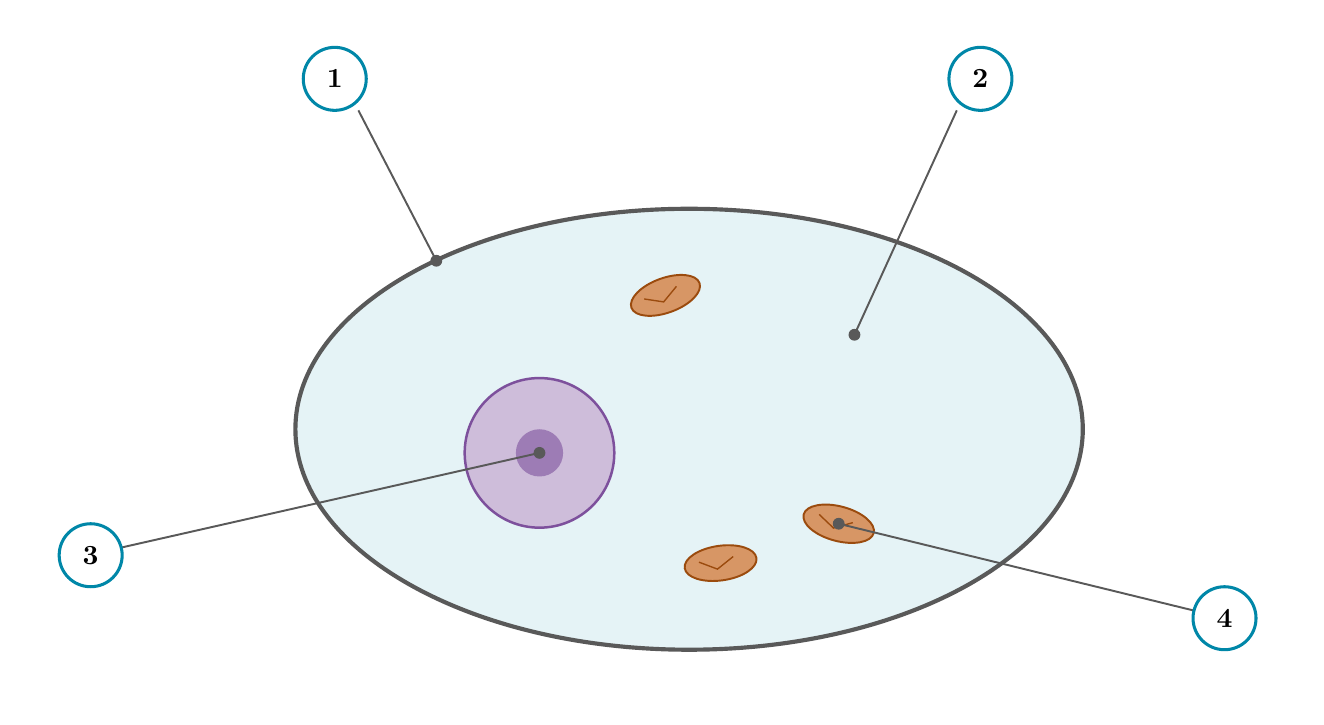
\begin{tikzpicture}[x=1cm,y=1cm,
    lbl/.style={circle, draw=cbteal, fill=white, line width=1.1pt,
                inner sep=1.8pt, minimum size=8mm, font=\bfseries}]

  % -- the cell. ONE outline only: an animal cell has a membrane and no wall,
  %    and drawing two edges here would teach exactly the wrong thing.
  \fill[cbteal!10] (5.5,3) ellipse (5.0 and 2.8);
  \draw[line width=1.5pt, black!65] (5.5,3) ellipse (5.0 and 2.8);

  % -- nucleus --
  \fill[cbpurple!30] (3.6,2.7) circle (0.95);
  \draw[line width=0.9pt, cbpurple!80] (3.6,2.7) circle (0.95);
  \fill[cbpurple!60] (3.6,2.7) circle (0.30);

  % -- mitochondria. Kept clear of (7.6,4.2) so the cytoplasm leader lands on an
  %    empty patch of cytoplasm and nothing else.
  % (5.2,4.7) rather than (3.0,4.5): a mitochondrion sitting just inside where
  % leader 1 lands makes the membrane leader ambiguous, which is the whole
  % question here.
  \foreach \x/\y/\r in {7.4/1.8/-15, 5.2/4.7/20, 5.9/1.3/8}{
    \begin{scope}[shift={(\x,\y)}, rotate=\r]
      \fill[cborange!65] (0,0) ellipse (0.46 and 0.22);
      \draw[line width=0.7pt, cborange!80!black] (0,0) ellipse (0.46 and 0.22);
      \draw[line width=0.5pt, cborange!80!black] (-0.27,0.05) -- (-0.05,-0.07) -- (0.17,0.06);
    \end{scope}}

  % -- leader lines. Every one ends on a dot, on the structure itself.
  \foreach \sx/\sy/\ex/\ey/\lx/\ly/\n in {%
      2.29/5.14/1.3/7.05/1.0/7.45/1,       % cell membrane (the outline)
      7.60/4.20/8.9/7.05/9.2/7.45/2,       % cytoplasm (empty patch)
      3.60/2.70/-1.7/1.5/-2.1/1.4/3,       % nucleus
      7.40/1.80/11.9/0.7/12.3/0.6/4}{      % mitochondrion
    \draw[line width=0.7pt, black!65] (\sx,\sy) -- (\ex,\ey);
    \fill[black!65] (\sx,\sy) circle (0.075);
    \node[lbl] at (\lx,\ly) {\n};}

  \path (-2.9,-0.4) rectangle (13.2,8.1);
\end{tikzpicture}}

\vspace{10pt}
\noindent
\begin{tabular}{@{}p{0.48\textwidth} p{0.48\textwidth}@{}}
  1.\ \blank[5.4cm] & 3.\ \blank[5.4cm] \\[14pt]
  2.\ \blank[5.4cm] & 4.\ \blank[5.4cm] \\
\end{tabular}

\vspace{10pt}
\noindent\textbf{Now think.} Name \textbf{two} things a \textbf{plant} cell would
have that this cell does not.
\wlines{2}

% ===========================================================================
% SECTION B -- MATHS: INTEGERS
% ===========================================================================
% This heading lands at the foot of page 3 and its rules box cannot follow it
% there. Guarding the pair with \needspace{15} pushes both over and costs a whole
% page; the cheaper fix is the line of prose below, which does fit, so the page
% ends on a sentence rather than on a bare heading.
\hwsection{Section B \textperiodcentered\ Mathematics 1.1--1.2 --- Integers}

\noindent The rules are on the next page. Try each question \key{before} you look at
them --- if you can, you know them.

\begin{remember}[The two sets of rules, side by side]
  {\renewcommand{\arraystretch}{1.2}%
  \begin{tabularx}{\linewidth}{@{}p{6.6cm}X@{}}
    Add a positive \sep move \key{right}      & $(+) \times (+) = (+)$ \\
    Add a negative \sep move \key{left}       & $(-) \times (-) = (+)$ \\
    Subtract a positive \sep move \key{left}  & $(+) \times (-) = (-)$ \\
    Subtract a negative \sep move \key{right} & $(-) \times (+) = (-)$ \\
  \end{tabularx}}

  % \smallskip, not \medskip. The packet sits exactly on the 8-page boundary and
  % 2mm here costs a whole page.
  \smallskip
  \key{Two negatives make a positive} is true for $\times$ and $\div$. It is
  \key{not} true for $+$: \; $-6 + (-4) = -10$, not $-2$.
\end{remember}

% -- B1 ---------------------------------------------------------------------
% The easy way in. There is no number-line diagram here on purpose: this is a
% review packet, the class has drawn the line four times, and the page it cost
% was needed for the word problems.
\qhead{B1}{Higher, lower, warmer, colder}

\noindent Complete each sentence with \eng{higher than}, \eng{lower than},
\eng{warmer than} or \eng{colder than}.

\begin{enumerate}[label=(\roman*)]
  \item $-9$ is \blank[3.4cm] $-2$.
  \item A temperature of $-1\dC$ is \blank[3.4cm] a temperature of $6\dC$.
  \item Floor $3$ is \blank[3.4cm] floor $-1$.
\end{enumerate}

% -- B2 ---------------------------------------------------------------------
\qhead{B2}{All four rules, and all four signs}

\noindent Work these out. You may draw a small number line beside any of them.

\vspace{9pt}
\begin{multicols}{3}
\begin{enumerate}[label=(\alph*), itemsep=13pt]
  \item $-7+3 = \blank[1.5cm]$
  \item $6+(-11) = \blank[1.5cm]$
  \item $-4-9 = \blank[1.5cm]$
  \item $-5-(-12) = \blank[1.5cm]$
  \item $-8 \times 3 = \blank[1.5cm]$
  \item $-6 \times (-7) = \blank[1.5cm]$
  \item $45 \div (-9) = \blank[1.5cm]$
  \item $-72 \div (-8) = \blank[1.5cm]$
  \item $-20+(-14) = \blank[1.5cm]$
  \item $12-(-12) = \blank[1.5cm]$
  \item $-4 \times (-5) \times (-2) = \blank[1.2cm]$
  \item $-30 \div 6 \times (-2) = \blank[1.2cm]$
\end{enumerate}
\end{multicols}

% -- B3 ---------------------------------------------------------------------
\qhead{B3}{Say it, then write it}

\begin{wordhelp}[Word help --- these words decide the order of your calculation]
  \begin{tabularx}{\linewidth}{@{}lX@{}}
    \eng{subtract 5 from 8}      & you \textbf{start} at 8: $8-5$. The English gives the numbers in the \textbf{opposite order} to the calculation. \\
    \eng{take 6 away from 2}     & the same trap: $2-6$. \\
    \eng{7 less than 3}          & again the same trap: $3-7$. \\
    \eng{owe} / \eng{a debt}     & money you must pay back. It makes your total \textbf{negative}. \\
    \eng{pay back}               & to give owed money \textbf{back}, so the debt gets \textbf{smaller}. \\
  \end{tabularx}
\end{wordhelp}

\noindent Turn each English sentence into a calculation, then work it out.
\key{Write the calculation first.}

\vspace{6pt}
\begin{enumerate}[label=\arabic*., itemsep=11pt]
  \item Subtract 11 from 5. \\[4pt]
        Calculation: \blank[6.2cm] \quad Answer: \blank[2.4cm]
  \item Take 8 away from $-3$. \\[4pt]
        Calculation: \blank[6.2cm] \quad Answer: \blank[2.4cm]
  \item What is 9 less than 2? \\[4pt]
        Calculation: \blank[6.2cm] \quad Answer: \blank[2.4cm]
  \item Mr Bowen owes 45 dollars. He pays back 20 dollars. \\[4pt]
        Calculation: \blank[6.2cm] \quad Answer: \blank[2.4cm]
\end{enumerate}

% -- B4 ---------------------------------------------------------------------
\qhead{B4}{Difference}

\begin{wordhelp}[Word help --- difference]
  The \eng{difference} between two numbers is the \textbf{gap} between them, so it is
  never negative --- and \eng{the difference between $a$ and $b$} is \textbf{not} the
  same instruction as \eng{$a$ minus $b$}. Question 2 is about exactly that.
\end{wordhelp}

\begin{enumerate}[label=\arabic*., itemsep=10pt]
  \item What is the difference between $12$ and $-5$? \blank[3.0cm]
  \item \textbf{(a)} The difference between $-7$ and $4$ is \blank[2.4cm]
        \qquad \textbf{(b)} $-7 - 4 = \blank[2.4cm]$ \\[6pt]
        \textbf{(c)} These two answers are not the same. Explain why.
        \wlines{2}
\end{enumerate}

% ===========================================================================
% SECTION C -- MATHS: FACTORS, MULTIPLES, TESTS, ROOTS
% ===========================================================================
\hwsection{Section C \textperiodcentered\ Mathematics 1.3--1.6 --- Factors, Multiples, Tests and Roots}

% -- C1 ---------------------------------------------------------------------
\qhead{C1}{Build the HCF and the LCM from the lists}

\begin{remember}[One list stops, the other never does]
  \key{Factors} divide into the number. That list \key{stops}, so we ask for the
  \key{highest} common one --- the \key{HCF}. \\
  \key{Multiples} are its times table. That list \key{never stops}, so we ask for the
  \key{lowest} common one --- the \key{LCM}.
\end{remember}

\noindent\textbf{(a)} All the factors of $48$: \blank[10.2cm]

\vspace{6pt}
\noindent\textbf{(b)} All the factors of $60$: \blank[10.2cm]

\vspace{6pt}
\noindent\textbf{(c)} The common factors: \blank[5.4cm] so the \key{HCF} is
\blank[2.2cm]

\vspace{9pt}
\noindent\textbf{(d)} The first six multiples of $8$: \blank[8.4cm]

\vspace{6pt}
\noindent\hspace*{1.2em}The first six multiples of $12$: \blank[8.2cm]

\vspace{6pt}
\noindent\hspace*{1.2em}So the \key{LCM} of 8 and 12 is \blank[2.6cm]

\vspace{9pt}
\noindent\textbf{(e)} A student says the LCM of 8 and 12 is 96, because
$8 \times 12 = 96$. Is 96 a common multiple of 8 and 12? Is it the \textbf{lowest}
one? Explain.
\wlines{2}

% -- C2 ---------------------------------------------------------------------
% The HCF/LCM confusion is the biggest language trap left in Unit 1, and HW 2 and
% HW 3 could only test the two one at a time. Side by side is where the class
% actually meets it, so this question is the point of Section C.
\qhead[cbgreen]{C2}{Which one does the question want?}

\begin{wordhelp}[Word help --- the words that tell you which tool to reach for]
  \eng{together again} \sep \eng{at the same time} \sep \eng{how often} --- something
  \textbf{repeating}. You want the \key{LCM}. \\
  \eng{share into equal groups} \sep \eng{as large as possible} \sep
  \eng{none left over} --- something being \textbf{split up}. You want the \key{HCF}.
\end{wordhelp}

\noindent Tick \textbf{HCF} or \textbf{LCM} for each one, then work out the answer.

\vspace{8pt}
\noindent
\begin{tabularx}{\textwidth}{|X|>{\centering\arraybackslash}p{1.5cm}|>{\centering\arraybackslash}p{1.5cm}|>{\centering\arraybackslash}p{2.6cm}|}
  \hline
  \textbf{The question} & \textbf{HCF} & \textbf{LCM} & \textbf{Answer} \\
  \hline
  One bell rings every 6 minutes, another every 10. They ring together now. In how
  many minutes will they ring together again? & & & \\
  \hline
  Mr Bowen has 24 pens and 36 pencils. He makes identical packs, using everything,
  with none left over. What is the greatest number of packs? & & & \\
  \hline
  Ribbons 45 cm and 60 cm long are cut into equal pieces, as long as possible, with
  none wasted. How long is each piece? & & & \\
  \hline
  A red bus leaves every 12 minutes and a blue bus every 18 minutes. They leave
  together at 7 am. When do they next leave together? & & & \\
  \hline
\end{tabularx}

% -- C3 ---------------------------------------------------------------------
\qhead{C3}{Tests for divisibility}

\noindent\textbf{(a)} Put a tick ($\checkmark$) where the number divides exactly.
Use the tests --- do \textbf{not} do the divisions.

\vspace{8pt}
\noindent
\begin{tabularx}{\textwidth}{|p{2.6cm}|X|X|X|X|X|X|}
  \hline
  \textbf{Number} & \textbf{2} & \textbf{3} & \textbf{4} & \textbf{5} & \textbf{6} & \textbf{9} \\
  \hline
  $3942$ \rule[-0.7em]{0pt}{2.1em} & & & & & & \\ \hline
  $5280$ \rule[-0.7em]{0pt}{2.1em} & & & & & & \\ \hline
  $7128$ \rule[-0.7em]{0pt}{2.1em} & & & & & & \\ \hline
  $2475$ \rule[-0.7em]{0pt}{2.1em} & & & & & & \\ \hline
\end{tabularx}

\vspace{11pt}
\noindent\textbf{(b)} \eng{Three sentences, one fact.} We know that $48 \div 6 = 8$
exactly. Fill in the three ways of saying so.

\vspace{7pt}
\noindent\hspace*{1.2em}(i) $6$ is a \blank[3.2cm] of $48$. \qquad
(ii) $48$ is a \blank[3.2cm] of $6$.

\vspace{8pt}
\noindent\hspace*{1.2em}(iii) $48$ is \blank[3.2cm] by $6$.

% -- C4 ---------------------------------------------------------------------
\qhead{C4}{Squares, cubes and roots}

\begin{remember}[Rooting is squaring run backwards]
  $9^2 = 81$, so $\sqrt{81} = 9$. \quad $4^3 = 64$, so $\sqrt[3]{64} = 4$. \quad And a
  square number can never end in \key{2, 3, 7 or 8}.
\end{remember}

\vspace{2pt}
\begin{multicols}{3}
\begin{enumerate}[label=(\alph*), itemsep=13pt]
  \item $7^2 = \blank[1.5cm]$
  \item $11^2 = \blank[1.5cm]$
  \item $4^3 = \blank[1.5cm]$
  \item $10^3 = \blank[1.5cm]$
  \item $\sqrt{81} = \blank[1.5cm]$
  \item $\sqrt{144} = \blank[1.5cm]$
  \item $\sqrt[3]{27} = \blank[1.5cm]$
  \item $\sqrt[3]{125} = \blank[1.5cm]$
  \item $6^2 + 3^3 = \blank[1.5cm]$
\end{enumerate}
\end{multicols}

\vspace{6pt}
\noindent\textbf{(j)} Two of these \textbf{cannot} be square numbers. Ring them, and
say how you know without doing any working.

\vspace{9pt}
\noindent\hspace*{1.2em}$2500$ \qquad $4832$ \qquad $6400$ \qquad $1007$
\wlines{2}

\vspace{2pt}
\noindent\textbf{(k)} \eng{Consecutive} numbers follow each other, like 5, 6, 7. The
consecutive pair whose squares are $64$ and $81$ is \blank[2.6cm]

% ===========================================================================
% SECTION D -- MATHS: WORD PROBLEMS
% ===========================================================================
\hwsection{Section D \textperiodcentered\ Mathematics --- Word Problems}

\noindent Every question here is one of the six maths lessons wearing a story. Before
you calculate, ask yourself \key{which lesson this is} --- then write the calculation
down before the answer.

\vspace{4pt}
\begin{enumerate}[label=\textbf{\arabic*.}, itemsep=11pt]

  \item \textbf{Sa Pa.} At 5 am the temperature was $-4\dC$. By 1 pm it had risen by
        13 degrees. By 9 pm it had fallen by 9 degrees.
        \textbf{(a)} What was the temperature at 9 pm?
        \textbf{(b)} What is the difference between the warmest and the coldest
        temperature of the day?
        \begin{workspace}[2.2cm]\end{workspace}

  \item \textbf{The lighthouses.} One lighthouse flashes every 8 seconds and another
        every 12 seconds. They flash together at exactly 9:00:00. At what time do
        they next flash together?
        \begin{workspace}[2.2cm]\end{workspace}

  \item \textbf{The pens.} Mr Bowen has 54 red pens and 36 blue pens. He makes
        identical packs, using every pen, with none left over, and he wants
        \textbf{as many packs as possible}. How many packs, and how many of each
        colour goes in one pack?
        \begin{workspace}[2.2cm]\end{workspace}

  \item \textbf{The patio.} \textbf{(a)} A square patio is made of 169 square tiles.
        How many tiles are there along one side?
        \textbf{(b)} A large cube is built from 216 small cubes. How many small
        cubes are there along one edge?
        \begin{workspace}[2.2cm]\end{workspace}

  % The deadpan one. Everything it needs was taught: the HCF, and then reading to
  % the end of the question before answering.
  \item \textbf{The biscuits.} Mr Bowen buys a bag of 60 round biscuits and a bag of
        48 square biscuits. He puts them on plates so that every plate has the same
        number of round biscuits and the same number of square biscuits, with none
        left over, using \textbf{as many plates as possible}.
        \textbf{(a)} How many plates are there?
        \textbf{(b)} How many biscuits are on one plate?
        \textbf{(c)} Mr Bowen then eats one whole plate. How many biscuits are left?
        \begin{workspace}[2.6cm]\end{workspace}

\end{enumerate}

% -- D2 ---------------------------------------------------------------------
\qhead[cbgreen]{D2}{Now you write the question}

\begin{yourturn}[The rules for both]
  A \textbf{real} situation --- money, temperature, floors, buses, packing. Full
  sentences, ending in a \textbf{question}. At least one of the \eng{signal words}
  from this packet. And your own question must actually come out at the answer given.
\end{yourturn}

\noindent Write a word problem for this calculation.

\vspace{7pt}
\noindent\hspace*{1.2em}\expr{-7 + 12 = 5}
\wlines{4}

% ===========================================================================
% ANSWER KEY (teacher copy only)
% ===========================================================================
\ifkey
\newpage
\hwsection[cbred]{Answer Key --- Teacher Copy}

\linespread{1.0}\selectfont
\setlist[enumerate]{itemsep=2pt, topsep=3pt, leftmargin=*}
\setlist[itemize]{itemsep=2pt, topsep=3pt, leftmargin=*}

\qhead[cbred]{A1}{Match the word to its meaning}
\noindent 1--D \quad 2--F \quad 3--H \quad 4--A \quad 5--C \quad 6--G \quad
7--E \quad 8--B

\smallskip
\noindent{\small The pair to watch is 2 and 3. A student who swaps \emph{tissue} and
\emph{organ} has the ladder upside down and will get A2 wrong as well --- mark the
two together and re-teach once, rather than twice.}

\qhead[cbred]{A2}{Climb the ladder}
\noindent
\begin{tabularx}{\linewidth}{@{}p{4.4cm}p{3.6cm}X@{}}
  A red blood cell     & cell         & tissue (blood) \\
  Muscle               & tissue       & organ (the heart, for example) \\
  The stomach          & organ        & organ system (the digestive system) \\
  The digestive system & organ system & organism \\
  Mr Bowen             & organism     & \textbf{nothing --- this is the top rung} \\
\end{tabularx}

\smallskip
\noindent{\small The last row is the question, and it is worth discussing rather than
marking. Most of the class will invent a rung --- ``a family'', ``a school'' ---
because the table has a box and a box wants filling. That instinct is the thing to
name out loud: \textbf{an empty box can be a correct answer}. Accept anything saying
there is no level above an organism.}

\qhead[cbred]{A3}{Name the cell}
\noindent (i) red blood cell \quad (ii) neurone / nerve cell \quad (iii) ciliated
cell \quad (iv) root hair cell \quad (v) palisade cell

\smallskip
\noindent (b) For example: ``A root hair cell is adapted to taking in water because it
has a long thin part that reaches into the soil.''

\smallskip
\noindent (c) A root hair cell is underground, where there is no light, so
chloroplasts would be no use to it. A palisade cell is near the top of the leaf where
the light is, and its job is to make food.

\smallskip
\noindent{\small In (b), mark the \emph{frame}, not the biology. The sentence must
contain both \emph{adapted to} + a job and \emph{because it has} + a feature. A
student who writes ``it has a long thin part'' has the science right and the sentence
wrong, and it is the sentence being taught here. \\
(c) separates recall from understanding. ``Because it does not need them'' is not yet
an answer --- push for \emph{no light underground}.}

\qhead[cbred]{A4}{Answer in full sentences}
\noindent A plant cell. The straight stiff edge is the cell wall, and the large space
in the middle is the sap vacuole; an animal cell has neither.

\smallskip
\noindent{\small This question wants the \emph{evidence}, not the verdict. ``Plant''
on its own is half an answer, and the missing half is the half being taught --- push
for both structures to be named, in sentences.}

\qhead[cbred]{A5}{Label the animal cell}
\noindent 1 --- cell membrane \quad 2 --- cytoplasm \quad 3 --- nucleus \quad
4 --- mitochondrion

\smallskip
\noindent \textbf{Now think:} any two of --- cell wall, chloroplasts, sap vacuole.

\smallskip
\noindent{\small Expect ``cell wall'' for 1. The diagram has one outline on purpose
and an animal cell has no wall, so this is a real error and not a slip: the outside of
an animal cell \emph{is} the membrane. That is the whole reason this packet labels an
animal cell rather than repeating the plant cell of Homework 1.}

\qhead[cbred]{B1}{Higher, lower, warmer, colder}
\noindent (i) lower than \quad (ii) colder than \quad (iii) higher than.

\smallskip
\noindent{\small The way in, and it should take a minute. If (i) goes wrong, the
number line is still not automatic and everything below it will be arithmetic done
by guesswork.}

\qhead[cbred]{B2}{All four rules, and all four signs}
\noindent (a) $-4$ \quad (b) $-5$ \quad (c) $-13$ \quad (d) $7$ \quad (e) $-24$
\quad (f) $42$ \\
(g) $-5$ \quad (h) $9$ \quad (i) $-34$ \quad (j) $24$ \quad (k) $-40$ \quad (l) $10$

\smallskip
\noindent{\small (i) is the whole point of putting the two rule sets side by side.
$-20+(-14)$ is an \textbf{addition}, so the two negatives do \textbf{not} make a
positive; a student who writes $34$ has over-applied the multiplying rule, and that
error deserves more class time than anything else on this page. \\
(k) has three negatives and comes out negative --- they cancel in pairs, and one is
left over. (l) must be worked left to right; a student who does $6 \times (-2)$ first
gets $2.5$ and should be shown why.}

\qhead[cbred]{B3}{Say it, then write it}
\begin{enumerate}[label=\arabic*., itemsep=3pt]
  \item $5-11=-6$
  \item $-3-8=-11$
  \item $2-9=-7$
  \item $-45+20=-25$
\end{enumerate}
\noindent{\small 1--3 are the reversed-order trap. If a student writes $11-5$,
$8-(-3)$ or $9-2$, that is an \textbf{English} error, not an arithmetic one --- do not
correct the sum, make them re-read the sentence and say which number they start at. \\
4 is the one to check: paying back a debt makes the total go \emph{up}, and a student
who writes $-45-20$ has read ``pays'' as ``spends''.}

\qhead[cbred]{B4}{Difference}
\noindent 1. $17$

\smallskip
\noindent 2. (a) $11$ \quad (b) $-11$ \quad (c) A difference is the gap between the
two numbers, so it is never negative. $-7-4$ is an instruction to start at $-7$ and
move 4 further left.

\smallskip
\noindent{\small Part (c) is the question. Accept any answer saying the first is a
\emph{distance} and the second is a \emph{move}. This is Homework 1's trap with new
numbers, and if the class still splits on it, it is worth ten minutes on the board
rather than a tick and a cross.}

\qhead[cbred]{C1}{Build the HCF and the LCM from the lists}
\noindent (a) $1, 2, 3, 4, 6, 8, 12, 16, 24, 48$ \\
(b) $1, 2, 3, 4, 5, 6, 10, 12, 15, 20, 30, 60$ \\
(c) $1, 2, 3, 4, 6, 12$; \; HCF $= \mathbf{12}$ \\
(d) $8, 16, 24, 32, 40, 48$ \; and \; $12, 24, 36, 48, 60, 72$; \; LCM $= \mathbf{24}$ \\
(e) 96 \emph{is} a common multiple --- $8 \times 12$ always is. It is not the
\textbf{lowest}, because 24 is smaller and is also in both lists.

\smallskip
\noindent{\small The common miss in (a) and (b) is a method problem. Students who hunt
in pairs ($1 \times 48$, $2 \times 24$, $3 \times 16$, $4 \times 12$, $6 \times 8$)
get all ten; students who count upwards in ones stop early and lose 16 and 24. Point
at the method, not the missing number. \\
(e) is worded so that ``yes'' and ``no'' are both needed. A student who answers only
``no'' has not read both questions.}

\qhead[cbred]{C2}{Which one does the question want?}
\noindent
\begin{tabularx}{\linewidth}{@{}p{6.0cm}p{2.0cm}X@{}}
  Two bells, 6 and 10 minutes   & \textbf{LCM} & 30 minutes \\
  24 pens and 36 pencils        & \textbf{HCF} & 12 packs (2 pens and 3 pencils in each) \\
  Ribbons 45 cm and 60 cm       & \textbf{HCF} & 15 cm each \\
  Buses every 12 and 18 minutes & \textbf{LCM} & 36 minutes, so 7:36 am \\
\end{tabularx}

\smallskip
\noindent{\small \textbf{Mark the ticks before the answers.} A right tick with wrong
arithmetic is a good piece of work; a wrong tick with tidy arithmetic is the error
this whole packet aims at. The give-away is size: a student who answers 2 minutes for
the bells, or 180 cm for the ribbon, has reached for the wrong tool --- and asking
``could a piece really be longer than the ribbon?'' fixes it faster than re-teaching
the method. \\
The bus question wants a \emph{time} back --- 7:36 am, not 36 --- because it asked
``when''. That is the same reading habit as everything in Section D.}

\qhead[cbred]{C3}{Tests for divisibility}
\noindent (a)
% The width is \linewidth less one tabcolsep pair: with @{} at both ends tabularx
% still counts the outer padding, and the table overhangs the text block by exactly
% 14pt. Shrinking the target width is the fix; widening the column is not.
\begin{tabularx}{\dimexpr\linewidth-14pt\relax}{@{}p{2.0cm}>{\raggedright\arraybackslash}X@{}}
  $3942$ & 2, 3, 6, 9 \quad {\small(digit sum 18; last two digits 42, not a 4)} \\
  $5280$ & 2, 3, 4, 5, 6 \quad {\small(digit sum 15, so 3 but not 9)} \\
  $7128$ & 2, 3, 4, 6, 9 \quad {\small(digit sum 18; 28 divides by 4)} \\
  $2475$ & 3, 5, 9 \quad {\small(odd, so no 2 --- and therefore no 6)} \\
\end{tabularx}

\smallskip
\noindent (b) (i) \textbf{factor} \quad (ii) \textbf{multiple} \quad
(iii) \textbf{divisible}

\smallskip
\noindent{\small In (a), the row to check is 2475: a student who ticks 6 has not
noticed that 6 needs \emph{both} 2 and 3, and 2475 is odd. \\
(b) is a language question wearing arithmetic, and it is the one most likely to be
left blank. Three sentences describe one fact, and the class does not yet believe
that.}

\qhead[cbred]{C4}{Squares, cubes and roots}
\noindent (a) 49 \quad (b) 121 \quad (c) 64 \quad (d) 1000 \quad (e) 9 \quad (f) 12
\quad (g) 3 \quad (h) 5 \quad (i) $36+27=63$

\smallskip
\noindent (j) $\mathbf{4832}$ and $\mathbf{1007}$ --- a square number never ends in 2,
3, 7 or 8. ($2500 = 50^2$ and $6400 = 80^2$.) \quad (k) $\mathbf{8}$ and $\mathbf{9}$.

\smallskip
\noindent{\small (i) is the one that goes wrong, and not because of the arithmetic:
students read $3^3$ as $3 \times 3$ and answer 45. Squaring and cubing look almost
identical on the page, which is exactly why the two lists were copied out separately.
\\ (j) rewards \emph{not} calculating, so praise the student who answered it in five
seconds. \emph{Consecutive} in (k) is the word the textbook uses without ever
explaining it.}

\qhead[cbred]{D1}{Word problems}
\begin{enumerate}[label=\arabic*., itemsep=3pt]
  \item (a) $-4+13-9=\mathbf{0\dC}$. \; (b) Warmest $9\dC$ at 1 pm, coldest $-4\dC$ at
        5 am: $9-(-4)=\mathbf{13}$ degrees.
  \item LCM of 8 and 12 is 24, so \textbf{9:00:24}.
  \item HCF of 54 and 36 is 18. \textbf{18 packs}, each with \textbf{3 red} and
        \textbf{2 blue}.
  \item (a) $\sqrt{169}=\mathbf{13}$ tiles. \; (b) $\sqrt[3]{216}=\mathbf{6}$ cubes.
  \item HCF of 60 and 48 is 12. (a) \textbf{12 plates}. (b) $5+4=\mathbf{9}$ biscuits.
        (c) $108-9=\mathbf{99}$ left.
\end{enumerate}
\noindent{\small The diagnosis is almost never the arithmetic. \\
\textbf{1(a)} comes out at $0\dC$, and that is the question: a student who wrote the
calculation down will trust it, and a student who did not will decide zero ``looks
wrong'' and change it. This is the question to make the write-it-first argument with.
\\ \textbf{2} must come back as a \emph{time}; ``24'' is an unfinished answer. \\
\textbf{3} asks two things and half the class will answer one. \\
\textbf{5} is three steps and the last one is a subtraction, not a division --- a
student who answers 12 or 9 stopped reading. Part (b) needs both halves,
$60 \div 12 = 5$ and $48 \div 12 = 4$; answering ``5'' is the same stopped-reading
error one step earlier.}

\qhead[cbred]{D2}{Now you write the question}
\noindent No single right answer. Check the conditions in this order:
\begin{enumerate}[label=\arabic*., itemsep=3pt]
  \item \textbf{Does the story start at $-7$?} It must \emph{begin} there, not arrive
        there --- the same ``which number comes first'' problem as B3, and the one
        most of them will get wrong.
  \item \textbf{Is there a signal word, and does it match?} The $+12$ needs an
        \emph{up} word: rises, deposits, climbs, pays back.
  \item \textbf{Full sentences, ending in a question?}
  \item \textbf{Does their own question actually come out at 5?}
\end{enumerate}

\smallskip
\noindent{\small One that works: ``The temperature in Sa Pa was $-7\dC$ at midnight.
By noon it had risen by 12 degrees. What was the temperature at noon?'' \\
A question that simply ends ``what is $-7+12$?'' has not done the task --- it is the
calculation copied out in words, and that is worth naming out loud rather than marking
wrong. This is the single best question on the packet for finding out who is reading
and who is pattern-matching, so it is worth reading four or five of them to the class.}

\fi

\end{document}
